\vspace{12pt}
\section{Measurements to Confirm Dopant Incorporation in the Films}
A well-established feature of PLD is the consistent stoichiometry transfer from ablation target to thin film. Accordingly, it is reasonable to expect that the dopants introduced in the bulk samples employed as targets in this research will also be incorporated in the thin films grown during PLD. A simple technique to verify this incorporation is energy-dispersive X-rays (EDX). Figure \ref{fig:EDX:Gd} shows an EDX spectrum obtained from a thin film grown from a 20 mol\% Gd doped target (which is 4 at.\%). The clear Gd emission lines confirm the incorporation of the dopant in the film. Compositional analysis on this sample shown in Table \ref{tab:film:edx:gd} indicates that for this target at 4 at.\% doping the film has 2 at.\% of Gd content. In order to carry out a more quantitative check, a representative set of spectra is also shown in Figure \ref{fig:EDX:Yb} for the incorporation of Yb \cite{ECamata2012}. The figure shows EDX of the BaZrO$_3$ films grown from ablating targets with three different nominal concentrations of Yb on MgO. A peak for Yb at approximately 1.5 keV is present in the EDX spectrum for all three samples. The appearance of Yb peaks confirms that Yb was successfully incorporated into each thin film. As pictured in Figure \ref{fig:EDX:Yb}, the peak intensity increases as the nominal Yb concentration in the ablation targets rises. This correlation of peak intensity with target concentrations of Yb strongly suggests that the actual concentration of Yb in the film is proportional to the nominal concentration of Yb in the targets. Using the intensity of the EDX peaks, an estimate of the actual mol\% of Yb in the films was determined. The obtained values of mol\% Yb in the films were 3.1 mol\%, 5.5 mol\%, and 8.8 mol\% in comparison with the nominal concentrations of the targets used of 5 mol\%, 10 mol\%, and 15 mol\%, respectively \cite{ECamata2012}. Therefore in each case it appears that some dopant may be lost in the ablation process, although uncertainty in the EDX analysis should be taken in mind with regard to the difference in composition from the doping levels of the targets. 
\begin{figure}
    \centering
    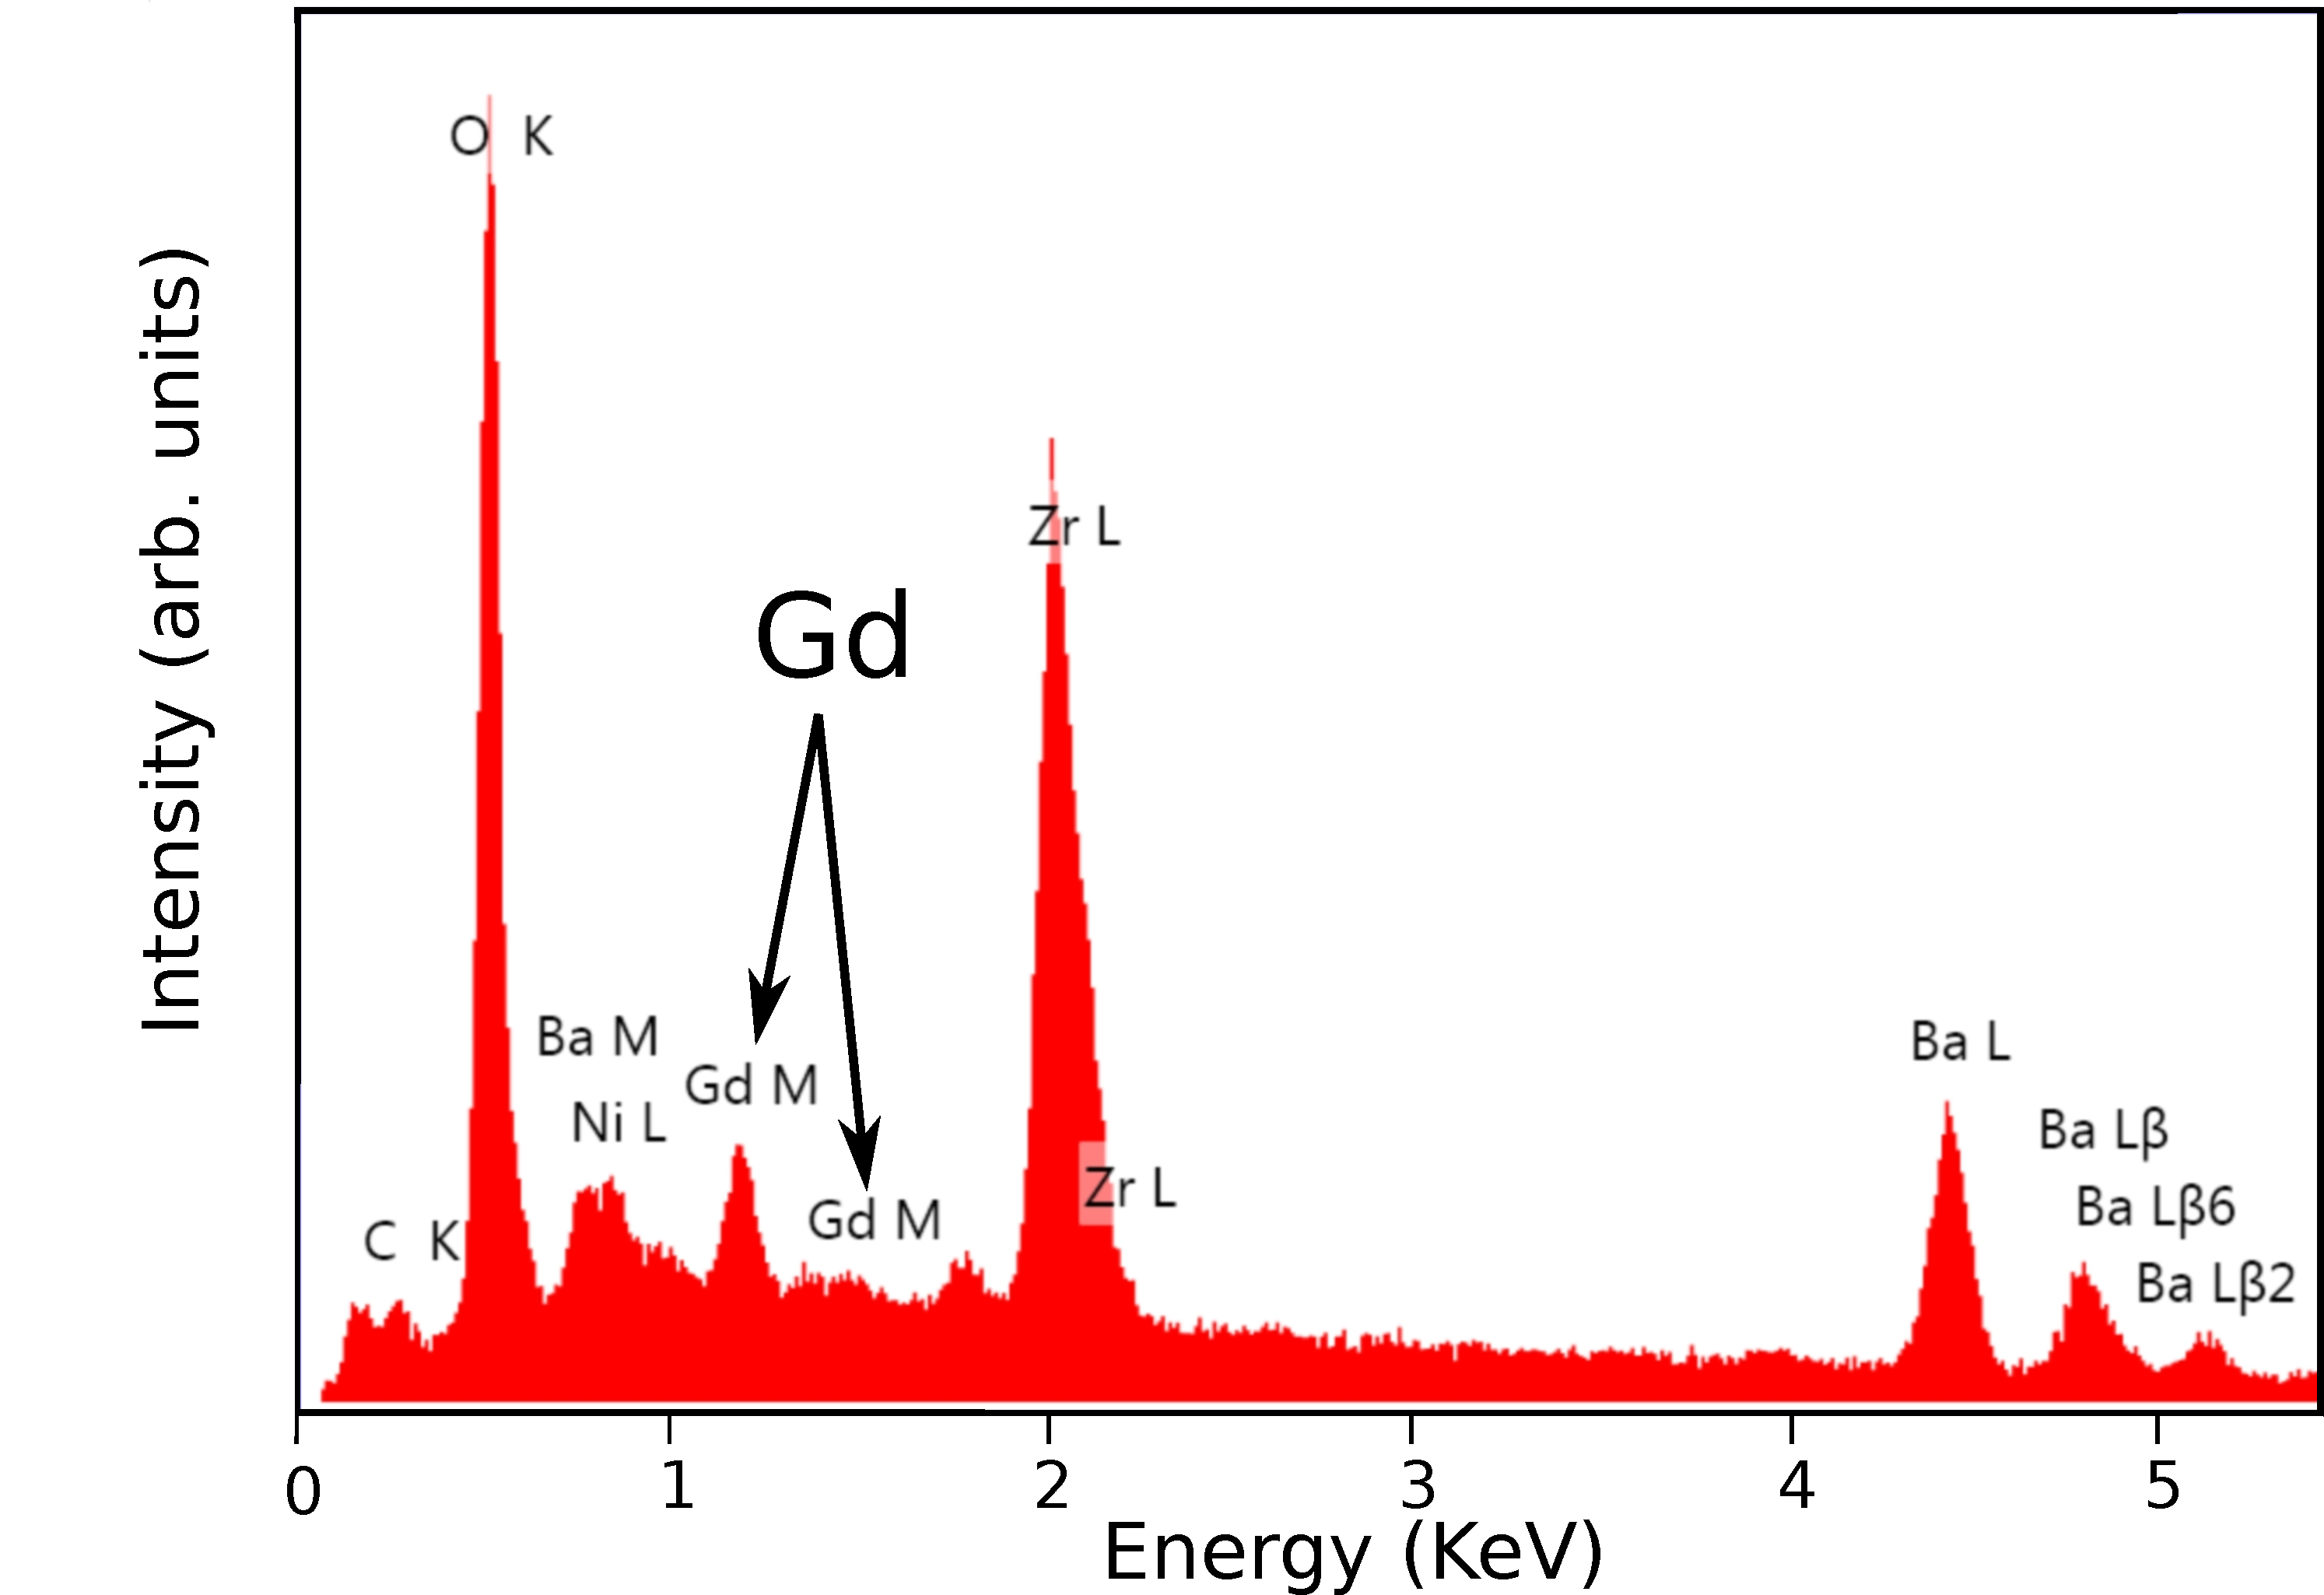
\includegraphics[width=.7\linewidth]{Figures/170714-edx-bzgxs10-mgo-edit.pdf}
    \caption{Energy-dispersive X-ray spectra on Gd:BaZrO\textsubscript{3} thin film deposited on MgO. The two gadolinium emission lines in the 1-2 KeV range confirm incorporation. Trace amounts of nickel are also present from contacts deposited nearby to the targeted scan area.}
    \label{fig:EDX:Gd}
\end{figure}

\begin{table}
    \centering
    \caption{Results of compositional analysis performed by EDX system on thin film of Gd:BaZrO\textsubscript{3} from a target made by solid state reaction initially doped with 4 at.\% gadolinium content.}
    \begin{tabular}{lr}
        \toprule
        Element &  Atomic \% \\
        \midrule
        \midrule
              O &      61.2 \\
             Ba &      21.5 \\
             Zr &      15.3 \\
             Gd &      2.01 \\
        \bottomrule
    \end{tabular}
    \label{tab:film:edx:gd}
\end{table}

% \begin{figure}
%     \centering
%     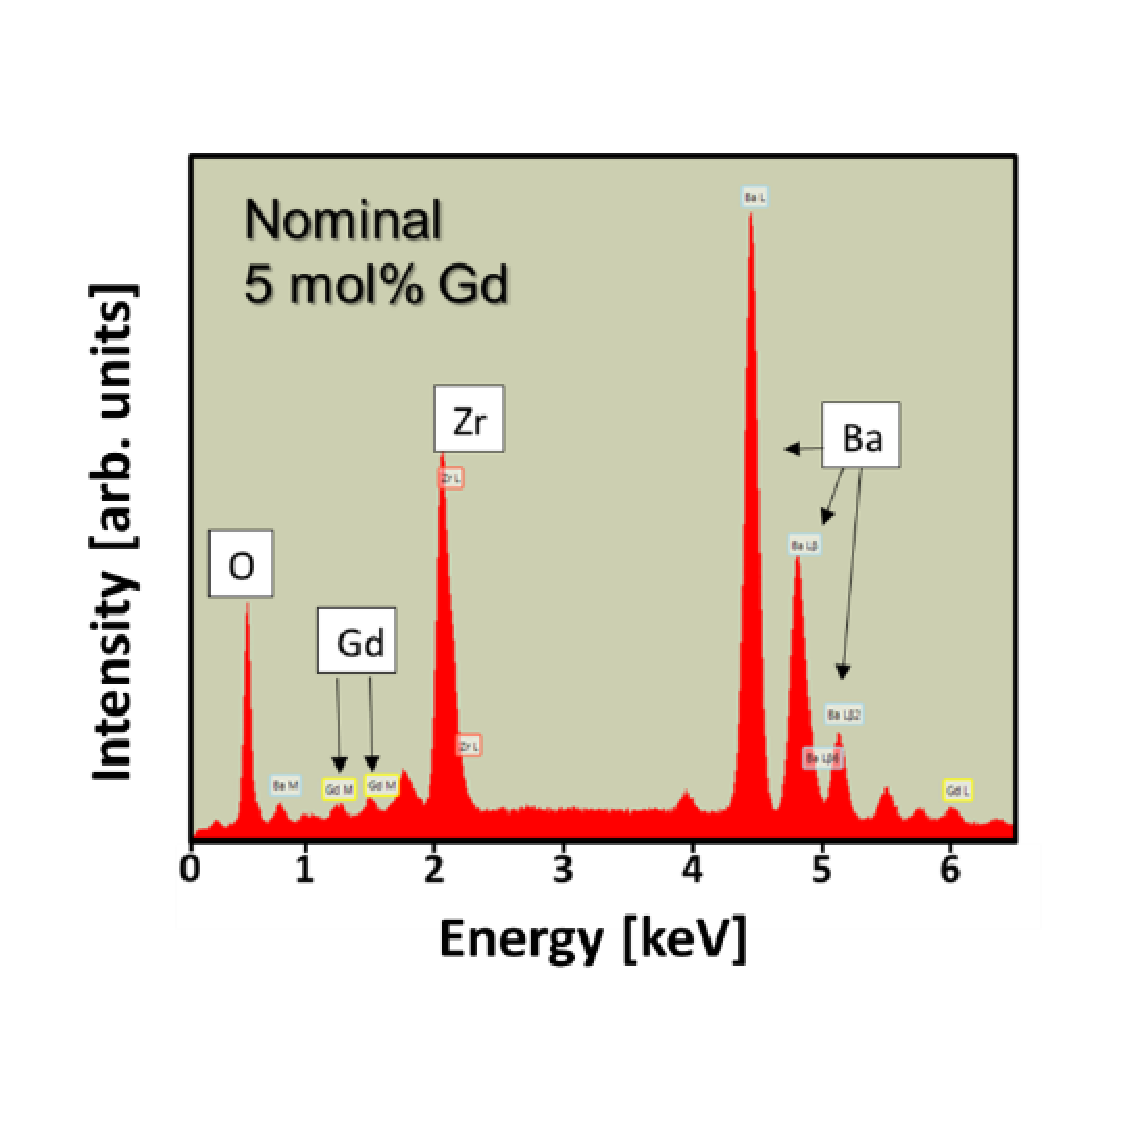
\includegraphics[width=0.7\textwidth]{Figures/EDX_Gd.pdf}
%     \caption{Energy-dispersive X-ray spectrum of a Gd-doped BaZrO$_3$ thin film with nominal dopant concentration of 5 wt. \%. The two Gd X-ray emission indicated in the 1-2 keV range confirm incorporation of Gd in the thin film.}
    
% \end{figure}

\begin{figure}
    \centering
    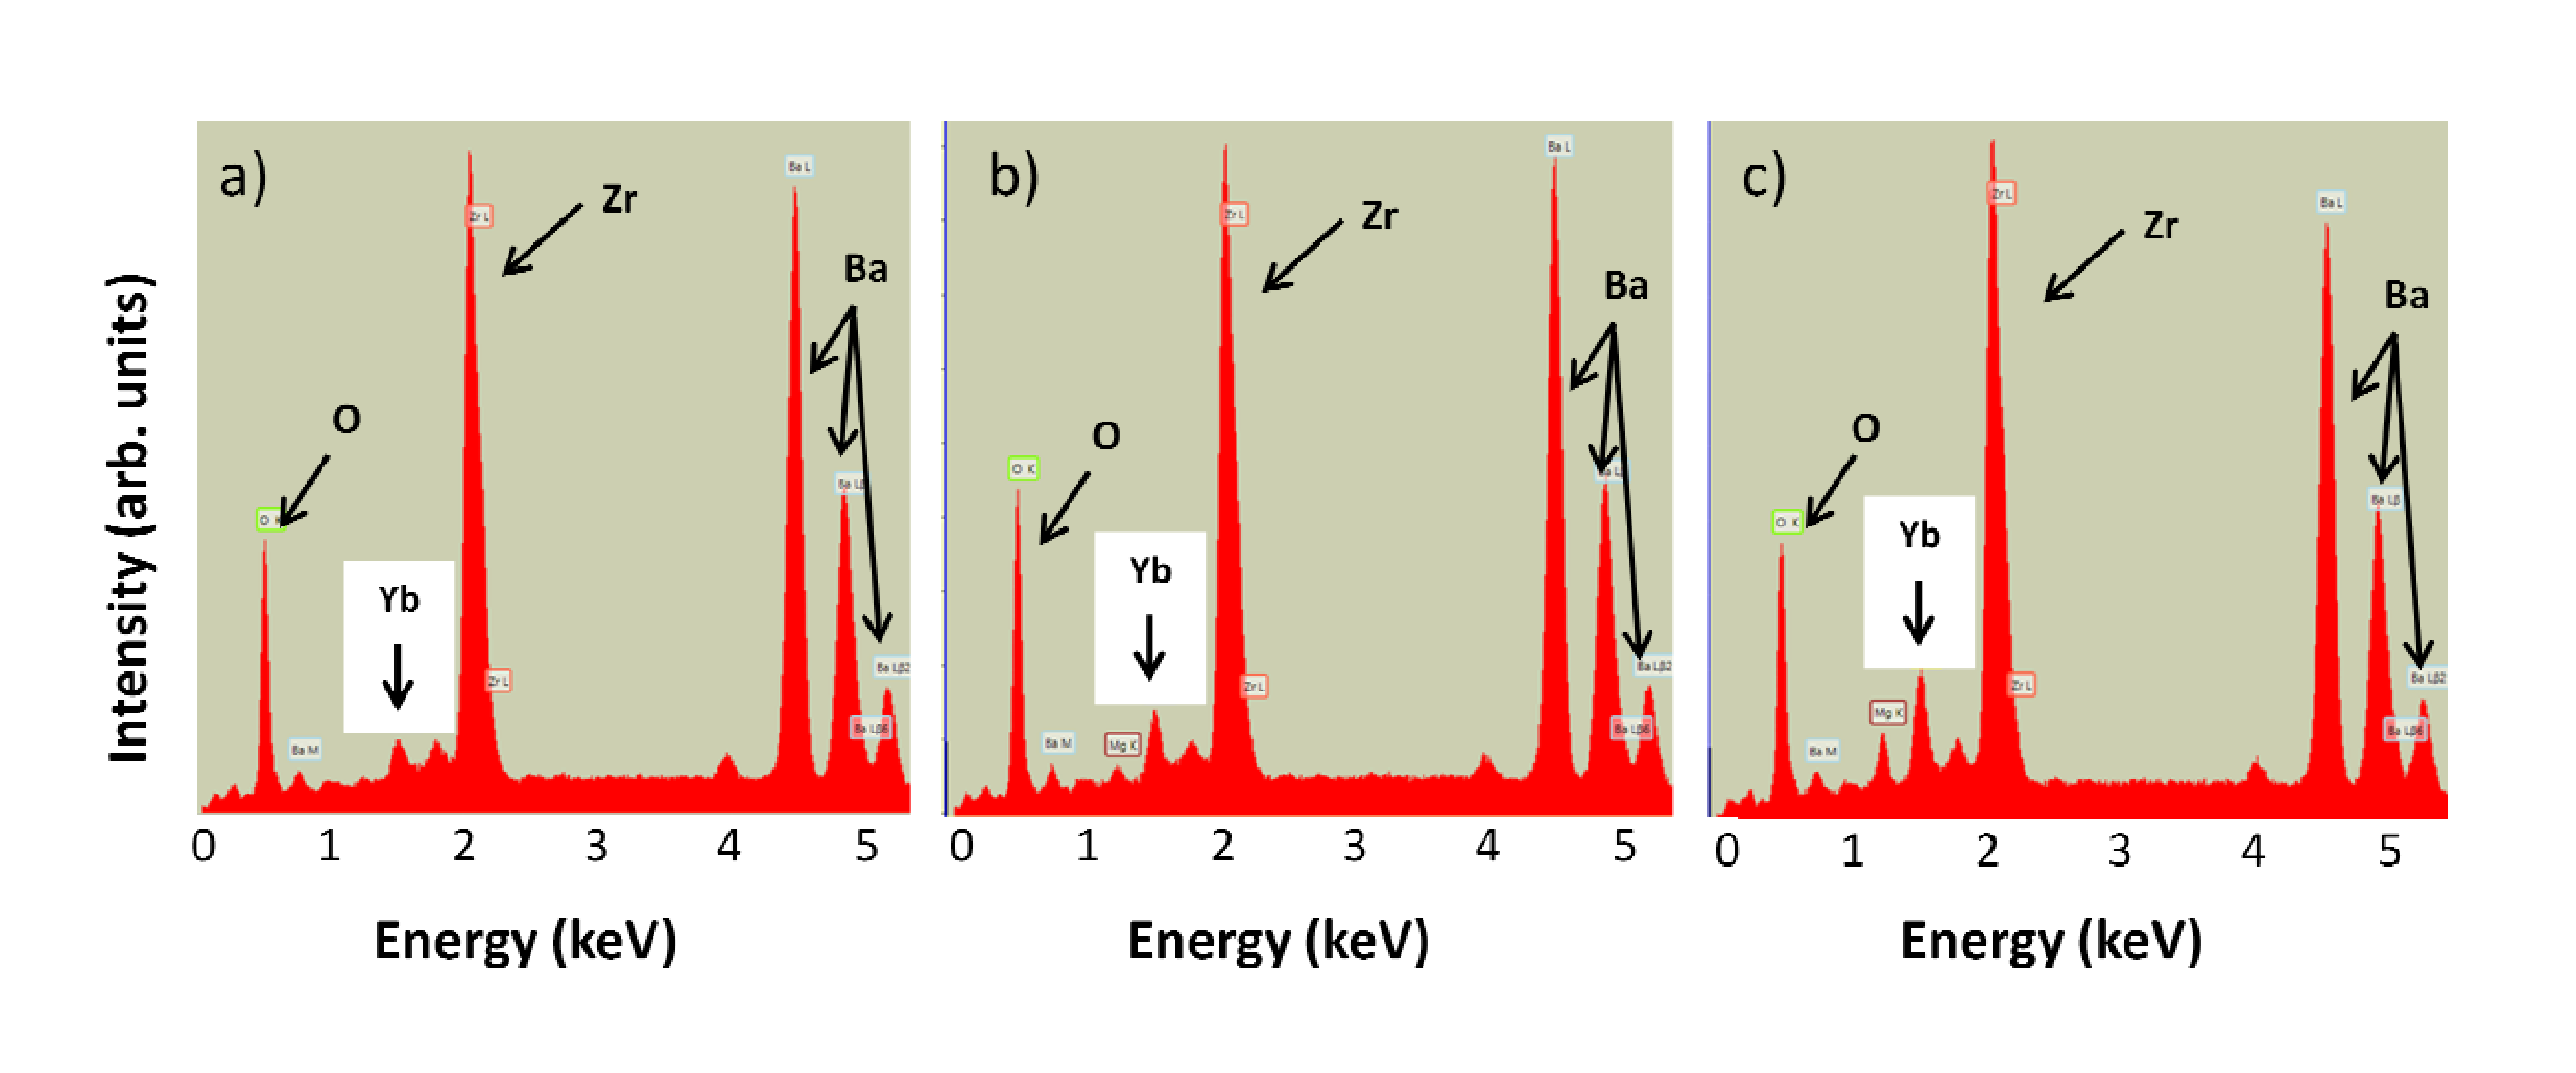
\includegraphics[width=\linewidth]{Figures/EDX_Yb.pdf}
    \caption{Energy-dispersive X-ray spectra of Yb-doped BaZrO$_3$ thin films. Data shows increasing EDX signal for the Yb emission as films were grown on MgO by ablating BaZrO$_3$ targets containing (a) 5 mol\% Yb, (b) 10 mol\% Yb, and (c) 15 mol\% Yb \cite{ECamata2012}.}
    \label{fig:EDX:Yb}
\end{figure}

